%%%%%%%%%%%%%%%%%%%%%%%%%%%%%%%%%%%%%%%%%
% University/School Laboratory Report
% LaTeX Template
% Version 3.1 (25/3/14)
%
% This template has been downloaded from:
% http://www.LaTeXTemplates.com
%
% Original author:
% Linux and Unix Users Group at Virginia Tech Wiki 
% (https://vtluug.org/wiki/Example_LaTeX_chem_lab_report)
%
% License:
% CC BY-NC-SA 3.0 (http://creativecommons.org/licenses/by-nc-sa/3.0/)
%
%%%%%%%%%%%%%%%%%%%%%%%%%%%%%%%%%%%%%%%%%

%----------------------------------------------------------------------------------------
%	PACKAGES AND DOCUMENT CONFIGURATIONS
%----------------------------------------------------------------------------------------

\documentclass{article}

\usepackage{graphicx} % Required for the inclusion of images
\usepackage{natbib} % Required to change bibliography style to APA
\usepackage{amsmath} % Required for some math elements 
\usepackage{amsthm}
\usepackage[hyphens]{url}
\usepackage{hyperref}
\usepackage{subcaption}
\usepackage{float}
\usepackage{array}
\usepackage{amssymb}


\setlength\parindent{0pt} % Removes all indentation from paragraphs

\newtheorem*{remark}{Theorem}
\newtheorem*{definition}{Definition}

%\renewcommand{\labelenumi}{\alph{enumi}.} % Make numbering in the enumerate environment by letter rather than number (e.g. section 6)

%\usepackage{times} % Uncomment to use the Times New Roman font

%----------------------------------------------------------------------------------------
%	DOCUMENT INFORMATION
%----------------------------------------------------------------------------------------

\title{Homework \#3 \\RSA \\[0.2em]\small{}CNS Course Sapienza} % Title and subtitle

\author{Riccardo \textsc{Prinzivalle}, 1904064} % Author name

\date{November 20, 2020} % Date for the report

\begin{document}

\maketitle % Insert the title, author and date

%----------------------------------------------------------------------------------------
%	SECTION 0
%----------------------------------------------------------------------------------------

\section{Homework Goal}

This homework contains an implementation of RSA algorithm based on major libraries for the mathematical functions, a comparison with the insecure \textit{PyCryptoDome} RSA and with the \textit{PyCryptoDome} AES.

%----------------------------------------------------------------------------------------
%	SECTION 1
%----------------------------------------------------------------------------------------

\section{RSA Implementation}

RSA basically is divided in two part: the initialization and the encryption.\newline 
The encryption phase is simpler than the initialization: it uses only an exponentiation and a modulo reduction. The modulo reduction is already implemented in python (used in this homework), instead what it is needed is an efficient implementation of the exponentiation. To do so, I used the proposed \textbf{Square And Multiply} in the slides of the course: at first with small values of base and exponent it worked flawlessly, but during the test with bigger messages and keys, the computation explodes, so I thought to reduce in modulo after every performed computation (since we have to do it after the exponentiation, so why don't do it at every step?) and the \textbf{SAM} computation time dropped to some seconds. The code can be seen in Fig. \ref{fig:sam}

\begin{figure}[H]
	\centering
	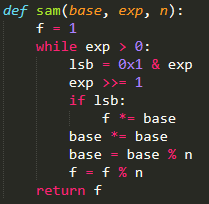
\includegraphics[width=0.345\linewidth]{images/SAM.png}
	\caption{Improved version of Square And Multiply}
	\label{fig:sam}
\end{figure}

Now the easy task is done; the initialization is the part which requires more attention to guarantee the security of our implementation. The operation to be performed are:

\begin{enumerate}
	\item find two large prime numbers $p$ and $q$
	\item compute $n = p \cdot q$
	\item compute Euler Phi function as $\Phi(n) = (p-1)(q-1)$ exploiting prime properties of $p$ and $q$
	\item select an exponent $e \in {1, 2, \dots, \Phi(n)}$ such that $gcd(e, \Phi(n) = 1$
	\item compute $d$ such that $d \cdot e = 1 \mod \Phi(n)$
\end{enumerate}

%----------------------------------------------------------------------------------------
%	SECTION 3
%----------------------------------------------------------------------------------------

\section{RSA Comparison}

\renewcommand{\arraystretch}{2}

\begin{table}[H]
	\begin{center}
		\begin{tabular}{ |c || c | c | c | c | c | c | }
			\hline
			Algorithm Family & Cryptosystems & \multicolumn{4}{c |}{Security Level (bit)}\\
			& & 80 & 128 & 192 & 256\\ [0.5ex] 
			\hline\hline
			Integer Factorization & RSA & 1024 & 3072 & 7680 & 15360  \\ 
			
			Discrete Logarithm & DH, DSA, Elgamal & 1024 & 3072 & 7680 & 15360  \\ 
			
			Elliptic Curves & ECDH, ECDSA & 160 & 256 & 384 & 512  \\ 
			\hline
			Symmetric key & AES, 3DES &  80 & 128 & 192 & 256  \\ 
			\hline
		\end{tabular}
		\caption{Key length comparison in public key and symmetric key algorithm}
		\label{tab:keyLen}
	\end{center}
\end{table}

%----------------------------------------------------------------------------------------
%	SECTION 4
%----------------------------------------------------------------------------------------

\section{Conclusion}

After this brief introduction on elliptic curves, it is obvious why they have been widely adopted in many cases of asymmetric encryption: they use less bits for the same level of security, so are more efficient to compute and their base concepts are easier to visualize. As suggested on section \ref{sec:use}, EC can be easily used in hybrid encryption scheme, in the key exchange phase.

%----------------------------------------------------------------------------------------
%	BIBLIOGRAPHY
%----------------------------------------------------------------------------------------

\bibliographystyle{abbrv}

\bibliography{biblio}

%----------------------------------------------------------------------------------------


\end{document}